\documentclass[10pt, a4paper, titlepage]{article}
%Kept only the packages needed
\usepackage{graphicx}  
\usepackage{subcaption} 
\usepackage{float}      

\begin{document}
\title{My first LaTeX attempt}
\author{Antonios Kagialis}
\date{September 2026}

%Question 1
\maketitle

%Question 2
\textit{Time for a random equation:}

In math, the area of the circle is \(A = \pi r^2\)
\newpage

%Question 3
\section{Bayesian Statistics}
Making an introduction to Bayesian statistics it is very important......
\subsection{Necessary readings}
Before moving forward with Bayesian stastics it is essential to read....
\newpage

%Question 4
\begin{figure}[H]
    \centering

    % Top left
    \begin{subfigure}[t]{0.47\textwidth}
        \centering
        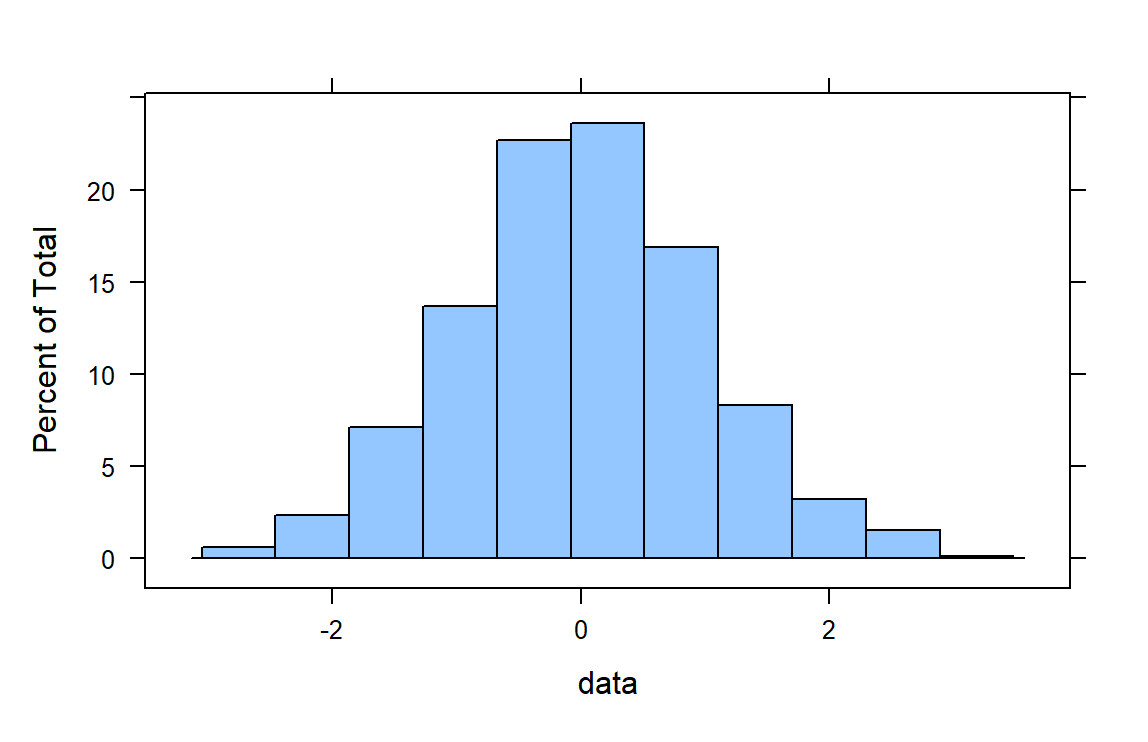
\includegraphics[width=\linewidth,height=4cm,keepaspectratio]{histogram.png}
        \caption{Histogram}
        \label{fig:histogram}
    \end{subfigure}
    \hfill
    % Top right
    \begin{subfigure}[t]{0.47\textwidth}
        \centering
        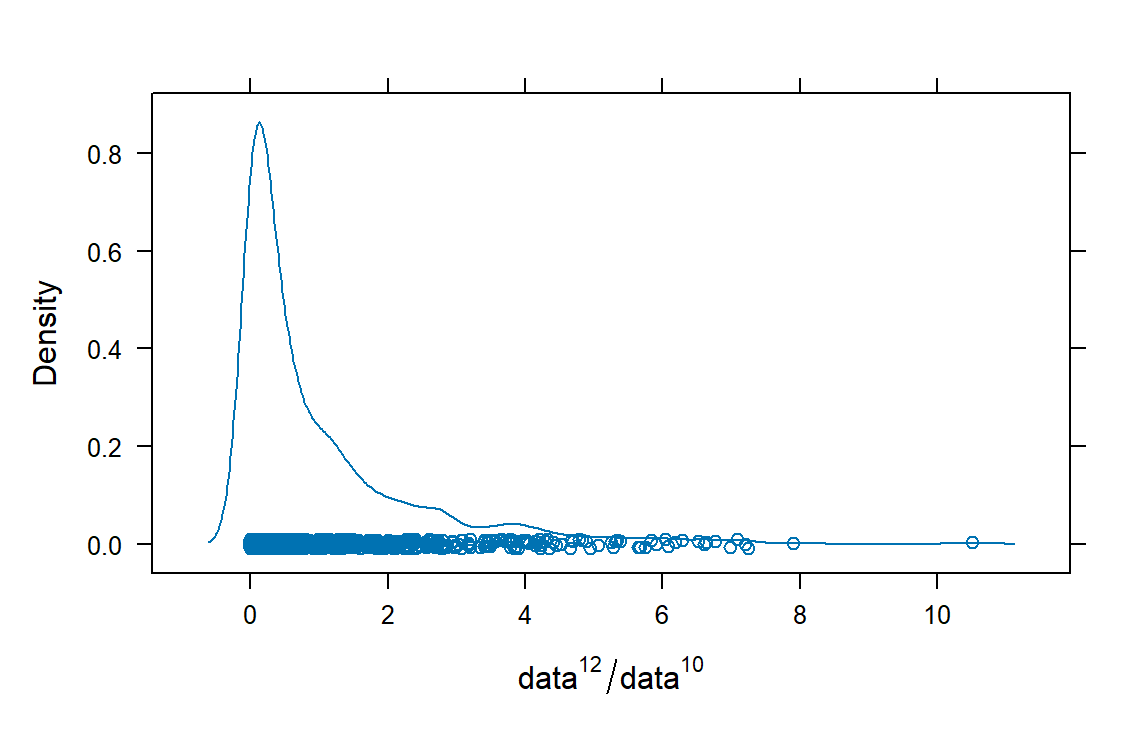
\includegraphics[width=\linewidth,height=4cm,keepaspectratio]{Densityplot.png}
        \caption{Densityplot}
        \label{fig:densityplot}
    \end{subfigure}

    \par\vspace{0.3cm}

    % Bottom left
    \begin{subfigure}[t]{0.47\textwidth}
        \centering
        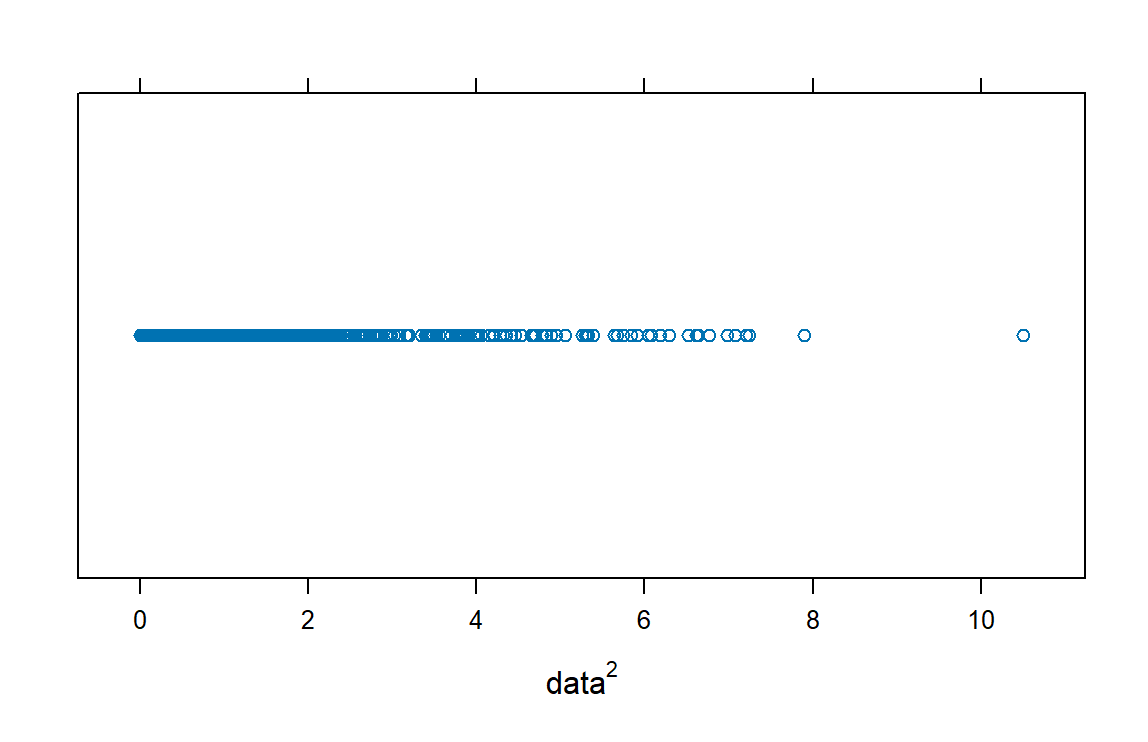
\includegraphics[width=\linewidth,height=4cm,keepaspectratio]{Stripplot.png}
        \caption{Stripplot}
        \label{fig:stripplot}
    \end{subfigure}
    \hfill
    % Bottom right
    \begin{subfigure}[t]{0.47\textwidth}
        \centering
        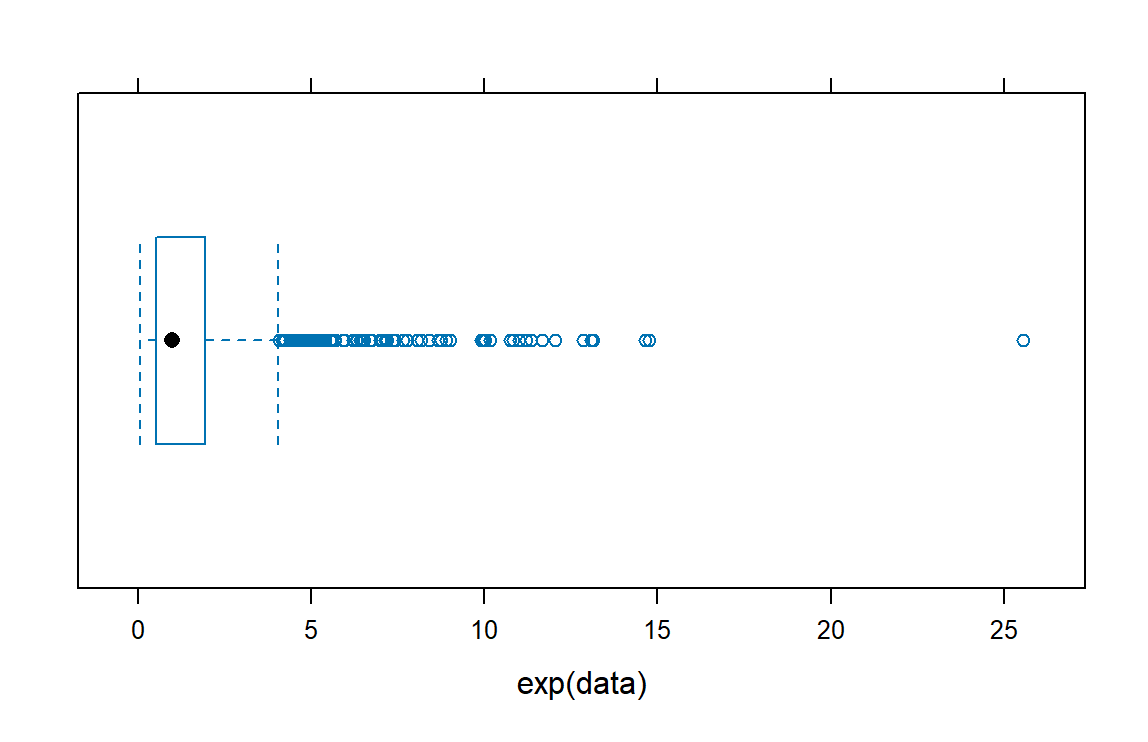
\includegraphics[width=\linewidth,height=4cm,keepaspectratio]{Boxplot.png}
        \caption{Boxplot}
        \label{fig:boxplot}
    \end{subfigure}

    \caption{Different plots of the same data, sometimes transformed. 
    No particular objective other than it being an exercise.}
    \label{fig:allplots}
\end{figure}

\vspace{0.3cm}

% latex table generated in R 4.6.1 by xtable 1.8-8 package
% Wed Sep  9 08:37:33 2026
\begin{table}[H]
\caption{The same data, but now in a table. Only the first nine rows are displayed.} 
\label{tab:data}
\centering
\begin{tabular}{rrrrr}
  \hline
 & data & squared1 & squared2 & exponent \\ 
  \hline
1 & -0.56 & 0.31 & 0.31 & 0.57 \\ 
  2 & -0.23 & 0.05 & 0.05 & 0.79 \\ 
  3 & 1.56 & 2.43 & 2.43 & 4.75 \\ 
  4 & 0.07 & 0.00 & 0.00 & 1.07 \\ 
  5 & 0.13 & 0.02 & 0.02 & 1.14 \\ 
  6 & 1.72 & 2.94 & 2.94 & 5.56 \\ 
  7 & 0.46 & 0.21 & 0.21 & 1.59 \\ 
  8 & -1.27 & 1.60 & 1.60 & 0.28 \\ 
  9 & -0.69 & 0.47 & 0.47 & 0.50 \\ 
   \hline
\end{tabular}
\end{table}
\newpage

%Question 5
\section{AI-generated fairytale}
\input{Clara.txt}

\end{document}

%Resources used
%https://www.overleaf.com/
% ChatGPT gave feedback on coding and recommedations to selected parts.
%All coding suggestions were reviewed by the author.